\documentclass{article}
\usepackage[utf8]{inputenc}
\usepackage{graphicx}
\usepackage{booktabs}
\usepackage[binary-units]{siunitx}
\usepackage[running]{lineno}
\usepackage{setspace}
\usepackage[]{authblk} % options: affil-it
\usepackage{natbib}
\usepackage{amsmath}
\usepackage{amssymb}
\usepackage{bm}
\usepackage{hyperref}
\usepackage{subcaption}
\usepackage{mathtools}

%\title{Fitting truncated generalized beta distributions to stem density data from permanent sample plots in Quebec, Canada}
\title{Diameter distribution models for Quebec, Canada}

\author{Gregory Paradis \thanks{Corresponding authour. Contact telephone number (418) 456-2208.}}
\affil{\footnotesize Département des sciences du bois et de la forêt, Faculté de foresterie, de géographie et de géomatique, Pavillon Abitibi–Price, Université Laval, Québec, QC G1K 7P4, Canada. \texttt{gregory.paradis.1@ulaval.ca}}

\author{Luc LeBel}
\affil{\footnotesize Département des sciences du bois et de la forêt, Faculté de foresterie, de géographie et de géomatique, Pavillon Abitibi–Price, Université Laval, Québec, QC G1K 7P4, Canada. \texttt{luc.lebel@sbf.ulaval.ca}}

\begin{document}
%\maketitle
\pagestyle{empty}

%\clearpage
% \begin{abstract}
% Statistical models predicting stem diameter distributions have found many applications in forestry.
% Our objective is to develop a methodology that can be used to derive a stem diameter distribution model for any combination of species and cover type in Quebec, Canada, using readily-available data from the government-run permanent sample plot inventory program. 
% We test 25 truncated distributions from the generalized beta family to a large dataset of stems inventoried from permanent fixed-area plots in the province of Quebec, Canada, using a non-linear least-squares parameter-fitting algorithm.
% We describe a two-stage parameter-fitting methodology that produces improved estimates of parameter estimation error and parameter correlation for input data with bounded domain.
% We report best-fit distribution, best-fit parameter estimates (with standard error on parameter estimates), and AICc for each of 30 subdatasets covering the entire province of Quebec (representing all combinations of 10 species groups and 3 cover types).
% Best-fit results are clearly dominated by the four distributions in the generalized gamma family. 
% \end{abstract}

%\linenumbers 
%\doublespace 

\clearpage
\section{Introduction}
\label{sec:introduction}

Stem diameter distributions (i.e. stand tables) have long played an important role in forestry \citep{bailey1973quantifying, hyink1983generalized}.
%The literature contains many examples of stem diameter distribution models.
Published models tend to be specific to a given combination of species, stand structure, geographic area, and inventory sampling method. 
No stem diameter distribution models have been published to date for the province of Quebec, Canada.
Furthermore, no generalized methodology has been published to model stem diameter distributions from permanent sample plot (PSP) data, documenting how to correctly estimate best-fit parameter uncertainty and correlations for the common case where observed diameter data has \emph{a priori} bounded domain (e.g. only merchantable stems of a certain minimum diameter are inventoried and trees never grow beyond a certain maximum diameter).
The present study fills these gaps in the literature.

The most commonly-used statistical model used to describe stem diameter seems to be the Weibull distribution \citep{bailey1973quantifying, liu2002finite, cao2004predicting, coomes2007mortality}. 
Other models include the gamma \citep{nelson1964diameter}, exponential \citep{meyer1943structure} and $S_B$ \citep{johnson1949systems} distributions.
The Weibull, gamma and exponential distributions are all derivatives of the generalized gamma distribution, which is itself a member of the of generalized beta family of statistical distributions.

We fit 25 truncated distributions from the generalized beta family to a large dataset of stems from government-compiled permanent fixed-area plots in the province of Quebec, Canada.
We describe a two-stage distribution-fitting methodology that correctly handles parameter estimation error and correlations for input data with bounded domain.
We present best-fit distributions for 30 combinations of species group and cover type.

Our best-fit distribution results cover all combinations of species and cover types in Quebec, and could be used directly.
Alternatively, our methodology can be easily replicated using readily-available PSP data, for example to derive models for different aggregations of species and cover type, or for a different geographic extent of plot data used as input.
The two-stage parameter-fitting methodology is potentially applicable to any context where trunctated data is fitted to standard-form statistical distributions.

The remainder of this paper is organized as follows.
We describe our methodology in \S\ref{sec:methods}. 
Results are presented in \S\ref{sec:results}, followed by discussion in \S\ref{sec:discussion}. % and concluding remarks in \S\ref{sec:conclusion}.

\section{Methods}
\label{sec:methods}

\citet{ducey2015sizebiased} document three parent distributions in the generalized beta family that can be used to derive several other distributions.
These parent distributions are the generalized beta distribution of the first kind (GB1), the generalized beta distribution of the second kind (GB2), and the generalized gamma distribution (GG).
The probability density functions (PDF) of GB1 and GB2 distributions have the following forms (adapted from \citealp{ducey2015sizebiased})
\begin{equation}
\text{GB1}(x; a, b, p, q) = \frac{|a|x^{ap-1}\left[1 - (x/b)^a\right]^{q-1}}{b^{ap}B(p, q)}, \qquad 0 < x^a < b^a, b > 0, p > 0, q > 0
\end{equation}
and 
\begin{equation}
\text{GB2}(x; a, b, p, q) = \frac{|a|x^{ap-1}x^{q-1}}{b^{ap}B(p, q)\left[1 - (x/b)^a\right]^{p+q}}, \qquad a > 0, b > 0, p > 0, q > 0
\end{equation}
defined for $x > 0$, where $\text{B}(p, q)$ represents the beta function (not to be confounded with the beta, or generalized beta, distributions), which is given by

\begin{equation}
\text{B}(p, q) = \int_0^1 t^{p-1} (1 - t)^{q-1} dt.
\end{equation}

The PDF of the generalized gamma GG distribution has the following form
\begin{equation}
\text{GG}(x; a, \beta, p) = \frac{ax^{ap-1}e^{-\left(\frac{x}{\beta}\right)^a}}{\beta^{ap}\Gamma(p)}, \qquad a > 0, \beta > 0, q > 0
\end{equation}
defined for $x > 0$, where $\Gamma(p)$ represents the gamma function (not to be confounded with the gamma, or generalized gamma, distributions), which is given by
\begin{equation}
\Gamma(p) = \int_0^\infty x^{p-1}e^{-x} dx.
\end{equation}

We can define the PDFs for 22 different distributions in the generalized beta family in terms of one of the three parent distributions, as follows (adapted from \citealp{ducey2015sizebiased})

\begin{align}
\text{IB1}(x; b, p, q) &= \text{GB1}(x; -1, b, p, q) \label{eq:distn_ib1} \\ 
\text{UG}(x; b, d, q) &= \lim_{a \to \infty} \text{GB1}(x; a, b, d/a, q) \\
\text{B1}(x; b, p, q) &= \text{GB1}(x; 1, b, p, q) \\
\text{B2}(x; b, p, q) &= \text{GB2}(x; 1, b, p, q) \\
\text{SM}(x; a, b, q) &= \text{GB2}(x; a, b, 1, q) \\
\text{Dagum}(x; a, b, p) &= \text{GB2}(x; a, b, p, 1) \\
\text{Pareto}(x; b, p) &= \text{GB1}(x; -1, b, p, 1) \\
\text{P}(x; b, p) &= \text{GB1}(x; 1, b, p, 1) \\
\text{LN}(x; \mu, \sigma) &= \lim_{a \to 0} \text{GG}(x; a, (\sigma^2 a^2)^{1/a}, (a\mu + 1)/(\sigma^2 a^2)) \\
\text{GA}(x; \beta, p) &= \text{GG}(x; 1, \beta, p) \\
\text{W}(x; a, \beta) &= \text{GG}(x; a, \beta, 1) \\
\text{F}(x; u, v) &= \text{GB2}(x; 1, v/u, u/2, v/2) \\
\text{L}(x; b, q) &= \text{GB2}(x; 1, b, 1, q) \\
\text{IL}(x; b, p) &= \text{GB2}(x; 1, b, p, 1) \\
\text{Fisk}(x; a, b) &= \text{GB2}(x; a, b, 1, 1) \\
\text{U}(x; b) &= \text{GB1}(x; 1, b, 1, 1) \\
\tfrac{1}{2}\text{N}(x; 0, \sigma) &= \text{GG}(x; 2, \sigma^2, 1/2) \\
\chi^2(x; p) &= \text{GG}(x; 1, 2, p) \\
\text{EXP}(x; \beta) &= \text{GG}(x; 1, \beta, 1) \\
\text{R}(x; \beta) &= \text{GG}(x; 2, \beta, 1) \\
\tfrac{1}{2}\text{t}(x; df) &= \text{GB2}(x; 2, \sqrt{df}, 1/2, df/2) \\
\text{LL}(x; b) &= \text{GB2}(x; 1, b, 1, 1) \label{eq:distn_ll}
\end{align}

We use a weighted non-linear least squares (NLLS) algorithm to fit target distributions to PSP inventory data binned into 26 size classes of uniform width $W$.

The objective function value of the NLLS problem minimizes the sum of squares of the residual terms
\begin{equation}
Z\left(f(x; \bm{\hat{P}})\right) = \text{min} \quad \sum_{\mathclap{i \in \{I|\hat{y}_i > 0\}}} e\left(f(x_i; \bm{P}), \hat{y}_i\right)^2 \label{eq:z}
\end{equation}
with
\begin{equation}
e\left(f(x_i; \bm{P}), \hat{y}_i\right) = w_i \left[f(x_i; \bm{P}) - \hat{y}_i\right] 
\end{equation}
where $x_i$ is the diameter corresponding to the center of bin $i \in I$, $f(x_i; \bm{P})$ is the value of the PDF of the target distribution at $x_i \in \bm{X}$ (given a vector of parameters $\bm{P}$). $\hat{y}_i \in \bm{\hat{Y}}$ represents the estimated stem density in bin $i$, which corresponds to the average of plot-wise stem density measurements.

Note that residual terms are scaled by a weight factor $w_i = 1 - \text{min}(E_{\hat{y}_i}\hat{y}_i^{-1}, 1)$, which dampens the impact of $\hat{y}_i$ on $Z$ as a function of the relative margin of error $E_{\hat{y}_i}\hat{y}_i^{-1}$. We cap relative margin of error at 1 (negative values of $w_i$ would have the effect of \emph{rewarding} large residual value $f(x_i; \bm{P}) - \hat{y}_i$, which would make NLLS algorithm results unnecessarily difficult to interpret).  
Thus, $w_i$ converges to 1 as relative margin of error approaches 0, and $w_i = 0$ if $E_{\hat{y}_i}\hat{y}_i^{-1} \geq 1$. 
Note that if sampling error is high enough for all bins (due to insufficient sample size), such that  $w_i = 0, \forall i \in I$, the objective function value is 0 regardless of values of input data vector $\bm{\hat{Y}}$ and the NLLS optimisation problem becomes meaningless.

The margin of error corresponds to the product $t\sigma_{\hat{y}_i}$ of the critical $t$ value (with $\alpha=0.05$ and $|\bm{\hat{Y}}|  - 1$ degrees of freedom) and bin-wise sampling error
\begin{equation}
\sigma_{\hat{y}_i}  = \sqrt{\frac{\sum_{j \in J} \left(y_{ij} - \hat{y}_i\right)^2}{|\bm{\hat{Y}}| - 1}}
\end{equation}
where $y_{ij}$ corresponds to the observed stem density in bin $i$ in sample plot $j$ \citep{schreuder2004statistical}.


We normalize our binned data, such that $\sum_{i \in I} W\hat{y}_i = 1$.
The domain of input data is bounded, such that $a \leq x_1 - w/2$ and $x_{|I|} + w/2 \leq b$, where $a > 0$.
Our dataset intentionally includes only merchantable stems (i.e.~$a =9$), and contains very few stems of diameter greater than 61 cm (i.e.~$b = 61$).

The integral of the standard forms of the PDFs described above over the interval $[0, \infty]$ is 1 for any given vector of input parameters $\bm{P}$, that is
\begin{equation}
\int_0^\infty f(x; \bm{P}) dx =  1.
\end{equation}

Fitting the standard forms of $f$ to the normalized binned data will generally produce poor fits, as the sum of residuals will be positively biased due to bounded domain (i.e.~$\sum_{i \in I} e_i>1$), with quality of fit inversely proportional to $b - a$.
We can obtain a better fit using an augmented PDF $f'(x; \bm{P'}) = sf(x; \bm{P})$.
The global scaling parameter $s$ effectively relaxes the unity constraint on the integral of $f'$.
Thus, using $f'$, we obtain similar quality fits for any scaling of bin value vector $\bm{\hat{Y}}$.

The variance $\sigma^2_{\hat{p}_j}$ of best-fit parameter estimator $\hat{p}_j \in \bm{\hat{P}}$ corresponds to element $j$ of the diagonal of the covariance matrix.
The covariance matrix, which is automatically calculated by most software implementations of the NLLS algorithm, corresponds to the inverse of the  negative of the expected values of the Hessian matrix $-E[H(\bm{\hat{P}})]$, where the Hessian $H(\bm{\hat{P}})$ is the matrix of second derivatives of the likelihood function $\mathcal{L}$ with respect to $\bm{\hat{P}}$.
Standard error $\sigma_{\hat{p}_j} = \sqrt{\sigma^2_{\hat{p}_j}}$ of parameter $\hat{p}_{j} \in \bm{\hat{P}}$ corresponds to the square root of the variance.

Note that variance estimates are only correct asymptotically.
In practice, fitting algorithms will use numerical approximations of Hessian matrix values.
Quality of finite approximations of the second derivatives of $\mathcal{L}$ will tend to be proportional to sample size $|\bm{\hat{Y}}|$, inversely proportional to distance from parameter constraint boundaries, and inversely proportional to the number of parameters $|\bm{\hat{P}}|$.

Parameter estimation error for augmented function  $f'(x; \bm{P'})$ can be improved, without deteriorating fit quality, by solving the fitting problem in two stages.
In the first stage, we determine $\bm{\hat{P'}}$ by solving for $Z(f'(x; \bm{\hat{P'}}))$.
For the best-case scenario, where $f'(x; \bm{P'})$ is fitted to an infinitely large sample $\bm{\hat{Y}}$ randomly drawn from $f'(x; \bm{\hat{P'}})$, the estimated value of scaling parameter $\hat{s} \in \bm{\hat{P'}}$ will completely eliminate the bias in the sum of residuals $\sum_{i \in I} e(f(x_i; \bm{\hat{P}}), \hat{y}_i)$, such that $\int_a^b f(x; \bm{\bar{P'}}) dx = \sum_{i \in I} W\hat{y}_i$.

In the second stage, we solve for  $Z(f''(x; \bm{\hat{P}}, \hat{s}))$, where $f''$ corresponds to our augmented distribution $f'$ with the scaling parameter value fixed at $s = \hat{s}$ (i.e.~only the original vector of parameters $\bm{P}$ is optimized by the fitting algorithm).

The shape distributions from both stages are equivalent, such that
\begin{equation}
 Z(f'(x; \bm{\hat{P'}})) \simeq Z(f''(x; \bm{\hat{P}}, \hat{s})). 
\end{equation}

However, error vector $\bm{\sigma}_{\hat{P}}$ and parameter covariance (which can be estimated from off-diagonal elements of the covariance matrix) estimated in the second stage will tend to be more reliable.

%%%%%%%%%%%%%%%

Our computational experiment dataset consists of 52~192 stems extracted from a database of PSP data, collected from public forests in Quebec (Canada). 
This data was collected by the \emph{Ministère de la forêt, de la faune et des parcs} (MFFP) as part of the official government inventory program\footnote{Detailed information on the
  PSP inventory program under which our test data was collected is available from the MFFP web site (\url{http://www.mffp.gouv.qc.ca/forets/inventaire/}).}, which operates on a 10-year cycle.

Data was collected throughout the province of Quebec, using 11.28 meter radius circular fixed-area plots.
The full dataset contains 1~685~233 stems, sampled from 12~570 permanent sample plot locations.
However, this includes repeated measures from four decennial inventory cycles, collected from 7 different PSP networks.
We filtered data to include only stems from the most recent inventory cycle, which ensures that we are not tallying repeated measures on the same plots.
We further filtered data to include only stems from the largest of the seven PSP networks (codename \emph{BAS1}), which ensures uniform data-collection standards for all stems.

Our ultimate goal (i.e.~beyond the scope of this paper) is to link a long-term wood supply optimization model with a short-term fibre-procurement optimization model.  
Thus, we are interested in modelling diameter distribution of merchantable stems in mature (operable), undisturbed stands.
We therefore applied a series of other filters to our stem dataset to exclude plots in disturbed or immature stands, unmerchantable stems (with DBH less than 9 cm), very large stems (with DBH greater than 61 cm), and dead or otherwise unmerchantable stems.

A Jupyter Notebook containing Python code implementing these filters and detailed explanations is available from the corresponding author upon request.
Although we do not have permission to distribute the PSP dataset, it is possible to request a copy from the \emph{Ministère des forêts, de la faune et de parcs} (see footnote for URL).

We segmented the 52~192 stems in our filtered PSP dataset into 30 sub-datasets, representing combinations of 10 species groups and 3 cover types.
More detailed information on species groups is provided in an appendix. 
For each of 30 sub-datasets $d \in D$, we applied our two-stage fitting method on 25 target distributions $f \in F$ (i.e. GB1, GB2, and GG parent distributions, and the 22 special cases of these distributions defined in (\ref{eq:distn_ib1}) through (\ref{eq:distn_ll})).

We used the small-sample form of the Akaike information criterion (AICc) to evaluate goodness-of-fit for each combination of $d \in D$ and $f \in F$. AICc is given by
\begin{equation}
\text{AICc} = AIC + \frac{2K(K + 1)}{n - K - 1}
\end{equation}
with 
\begin{equation}
\text{AIC} = 2K - n\ln\left(\frac{\chi^2}{n}\right)
\end{equation}
where $K=|\mathbf{P}|+1$ (i.e. the cardinality of the parameter vector $\mathbf{P}$, plus the $\mu$ parameter of the implicit i.i.d. Gaussian error distribution of input data vector $\mathbf{\hat{Y}}$), $n=|\mathbf{\hat{Y}}|$, as recommended in \citealp{burnham2002model}), and $\chi^2$ is the sum of squared residuals given by
\begin{equation}
\chi^2 = \sum_{i \in I} e\left(f(x_i; \bm{\hat{P}}), \hat{y}_i\right)^2
\end{equation}

For each sub-dataset $d \in D$, we ranked distributions $f \in F$ in decreasing order of AICc, and reported best-fit distribution, best-fit parameter values (with standard error estimates on parameter values) for first and second stages, and second-stage AICc.

\section{Results}
\label{sec:results}

Figures \ref{fig:results1} and \ref{fig:results2} show best-fit distributions plotted against empirical input data distribution, binned by diameter class. The name of the best-fit distribution is identified in the legend for each subplot.

Table \ref{tab:results} reports estimated parameter values, standard error on parameter estimates, and second-stage AICc for best-fit distributions. 


\begin{figure}[h!]
  \centering
  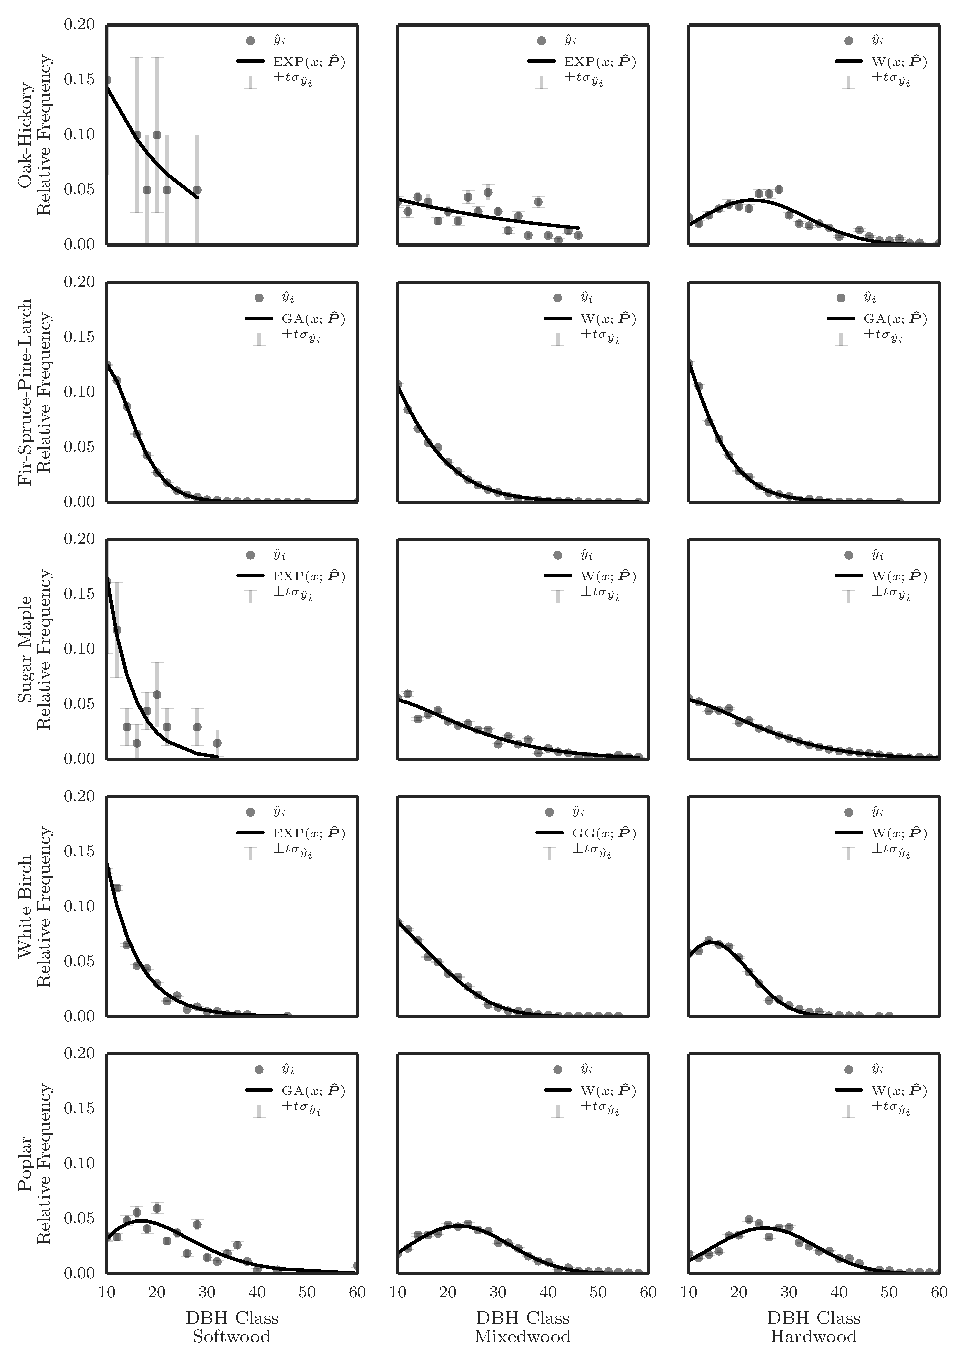
\includegraphics[width=1.0\textwidth]{images/pspdistfit_fitplot0}
  \caption{Best-fit distributions are shown with a solid
    line. Empirical distributions (binned by 2-cm
    diameter class) are shown with gray circles. Bin-wise sampling error is shown with light gray error bars. Species group is fixed for a given row of subfigures, and cover type is fixed for a given column of subfigures.}
  \label{fig:results1}
\end{figure}

\begin{figure}[h!]%\ContinuedFloat
  \centering
  \includegraphics[width=1.0\textwidth]{images/pspdistfit_fitplot1}
  \caption{(Continued from Figure \ref{fig:results1}) Best-fit distributions are shown with a solid
    line. Empirical distributions (binned by 2-cm diameter class) are shown with gray circles. Bin-wise sampling error is shown with light gray error bars. Species group is fixed for a given row of
    subfigures, and cover type is fixed for a given column of subfigures.}
  \label{fig:results2}
\end{figure}



\begin{table}
\caption{Best-fit distributions for each combination of species group
  and cover type. We report estimated parameter values and standard
  error for first- and second-stage fits, and second-stage AIC.}
\label{tab:results}
{\footnotesize
\begin{tabular}{lllllr}
\toprule
Species Group & Cover & Dist. & Parameters & Parameters & AICc \\
& Type & Name & (Stage 1) & (Stage 2) & (Stage 2) \\
\midrule
Oak-Hickory & S & EXP & $\beta$ = 20.83$\pm$3.22 & $\beta$ = 15.00$\pm$2.62 & -62 \\
 & M & EXP & $\beta$ = 40.80$\pm$15.09 & $\beta$ = 36.27$\pm$6.54 & -178 \\
 & H & W & a = 2.67$\pm$0.20 & a = 2.67$\pm$0.16 & -250 \\
 &  &  & $\beta$ = 27.09$\pm$0.80 & $\beta$ = 27.10$\pm$0.74 &  \\
Fir-Spruce-Pine-Larch & S & GA & $\beta$ = 2.35$\pm$0.04 & $\beta$ = 2.35$\pm$0.01 & -336 \\
 &  &  & p = 4.97$\pm$0.09 & p = 4.97$\pm$0.02 &  \\
 & M & W & a = 1.25$\pm$0.06 & a = 1.25$\pm$0.01 & -302 \\
 &  &  & $\beta$ = 10.63$\pm$0.44 & $\beta$ = 10.63$\pm$0.13 &  \\
 & H & GA & $\beta$ = 4.09$\pm$0.32 & $\beta$ = 4.09$\pm$0.09 & -253 \\
 &  &  & p = 2.42$\pm$0.27 & p = 2.42$\pm$0.04 &  \\
Sugar Maple & S & EXP & $\beta$ = 6.34$\pm$1.44 & $\beta$ = 5.20$\pm$0.35 & -79 \\
 & M & W & a = 1.33$\pm$0.14 & a = 1.35$\pm$0.06 & -274 \\
 &  &  & $\beta$ = 19.13$\pm$0.99 & $\beta$ = 19.20$\pm$0.89 &  \\
 & H & W & a = 1.42$\pm$0.06 & a = 1.42$\pm$0.02 & -328 \\
 &  &  & $\beta$ = 19.06$\pm$0.38 & $\beta$ = 19.06$\pm$0.35 &  \\
White Birch & S & EXP & $\beta$ = 6.24$\pm$0.39 & $\beta$ = 6.23$\pm$0.17 & -163 \\
 & M & GG & a = 2.78$\pm$0.57 & a = 2.77$\pm$0.22 & -289 \\
 &  &  & $\beta$ = 23.60$\pm$2.57 & $\beta$ = 23.57$\pm$0.56 &  \\
 &  &  & p = 0.25$\pm$0.14 & p = 0.25$\pm$0.03 &  \\
 & H & W & a = 2.55$\pm$0.08 & a = 2.55$\pm$0.05 & -238 \\
 &  &  & $\beta$ = 17.67$\pm$0.18 & $\beta$ = 17.67$\pm$0.17 &  \\
Poplar & S & GA & $\beta$ = 4.85$\pm$1.41 & $\beta$ = 4.73$\pm$0.85 & -170 \\
 &  &  & p = 4.46$\pm$1.17 & p = 4.55$\pm$0.79 &  \\
 & M & W & a = 2.76$\pm$0.07 & a = 2.76$\pm$0.05 & -311 \\
 &  &  & $\beta$ = 26.06$\pm$0.23 & $\beta$ = 26.06$\pm$0.22 &  \\
 & H & W & a = 3.03$\pm$0.15 & a = 3.03$\pm$0.12 & -285 \\
 &  &  & $\beta$ = 28.77$\pm$0.50 & $\beta$ = 28.77$\pm$0.48 &  \\Pine & S & GG & a = 5.17$\pm$2.62 & a = 5.15$\pm$2.39 & -277 \\
 &  &  & $\beta$ = 50.91$\pm$3.40 & $\beta$ = 50.83$\pm$2.40 &  \\
 &  &  & p = 0.20$\pm$0.14 & p = 0.20$\pm$0.12 &  \\
 & M & EXP & $\beta$ = 49.73$\pm$12.38 & $\beta$ = 46.81$\pm$5.81 & -264 \\
 & H & EXP & $\beta$ = 9.94$\pm$1.58 & $\beta$ = 9.93$\pm$1.16 & -159 \\
Other Hardwoods & S & GA & $\beta$ = 0.42$\pm$0.11 & $\beta$ = 0.43$\pm$0.07 & -101 \\
 &  &  & p = 28.54$\pm$7.58 & p = 28.08$\pm$4.80 &  \\
 & M & EXP & $\beta$ = 9.15$\pm$0.49 & $\beta$ = 9.15$\pm$0.34 & -208 \\
 & H & EXP & $\beta$ = 9.38$\pm$0.67 & $\beta$ = 9.41$\pm$0.48 & -253 \\
Other Maples & S & $\chi^2$ & p = 5.95$\pm$0.21 & p = 5.95$\pm$0.18 & -145 \\
 & M & GA & $\beta$ = 3.35$\pm$0.19 & $\beta$ = 3.35$\pm$0.09 & -288 \\
 &  &  & p = 4.45$\pm$0.26 & p = 4.45$\pm$0.12 &  \\
 & H & GA & $\beta$ = 4.91$\pm$0.48 & $\beta$ = 4.90$\pm$0.20 & -258 \\
 &  &  & p = 3.18$\pm$0.33 & p = 3.18$\pm$0.13 &  \\
Yellow Birch & S & EXP & $\beta$ = 20.20$\pm$2.75 & $\beta$ = 20.04$\pm$2.61 & -223 \\
 & M & B1 & b = 60.60$\pm$3.82 & b = 60.62$\pm$3.41 & -300 \\
 &  &  & p = 0.39$\pm$0.15 & p = 0.40$\pm$0.02 &  \\
 &  &  & q = 1.73$\pm$0.30 & q = 1.74$\pm$0.16 &  \\
 & H & EXP & $\beta$ = 16.60$\pm$1.34 & $\beta$ = 16.60$\pm$1.31 & -269 \\
Eastern White Cedar & S & W & a = 1.70$\pm$0.07 & a = 1.70$\pm$0.04 & -317 \\
 &  &  & $\beta$ = 20.42$\pm$0.37 & $\beta$ = 20.42$\pm$0.36 &  \\
 & M & GG & a = 2.87$\pm$0.94 & a = 2.83$\pm$0.45 & -307 \\
 &  &  & $\beta$ = 37.52$\pm$4.50 & $\beta$ = 37.34$\pm$1.28 &  \\
 &  &  & p = 0.16$\pm$0.13 & p = 0.17$\pm$0.03 &  \\
 & H & EXP & $\beta$ = 7.75$\pm$0.87 & $\beta$ = 7.67$\pm$0.49 & -182 \\
\bottomrule
\end{tabular}
}%
\end{table}

\section{Discussion}
\label{sec:discussion}

As predicted, second-stage parameter standard error estimates are systematically lower than first-stage error estimates.
This is attributable to fixing of the $s$ parameter in the second stage. 

Four distributions (GG, GA, W, EXP) dominate our best-fit model selection experiment, taking first place for 28 out of 30 combinations of species group and cover type. 
The $\chi^2$ and B1 distributions had the lowest AICc value for the other two cases.

This confirms previous results in the forestry literature reporting success using GG, GA, W, and EXP distributions to model stem diameter distribution from stem tally data.
If analytic resources are highly constrained, we recommend limiting the list of candidate distributions these four.
Note that in most cases many of the other 21 distributions were rejected altogether, either because the NLLS algorithm did not converge, or because fitting results were deems unstable (due to extremely high parameter values, or extremely high or otherwise unreliable parameter error estimates).
GA, W, and EXP distributions are all derivatives of the GG distribution, with one or more of its three parameters fixed to a value of 1. 
It is not surprising that the GG distribution generally had slightly better fit (i.e. lower $\chi^2$), however results show that AICc recommends selecting a more parsimonious model in most (but not all) cases.

Overall, fit results are very good, as indicated by relatively low second-stage parameter standard error estimates.
This observation can be confirmed by visual inspection of fit results in Figures \ref{fig:results1} and \ref{fig:results2}.
Relatively small sample sizes in some combinations of species group and cover type yielded binned datasets with more erratic values (including empty bins, which were excluded from NLLS algorithm input data before fitting).
Naturally, best-fit parameter standard error and AIC values are higher for these datasets. 

Our input dataset includes a large number of stems, inventoried throughout the province of Quebec.
Our best-fit distribution results could be used to forecast diameter distribution for mature stands in Quebec, or in other locations with similar forests.
For researchers looking for more customized fits, our two-stage methodology can easily be replicated on publicly-available inventory data.

% \section{Conclusion}
% \label{sec:conclusion}

% We tested 25 distributions in the generalized beta family, several of which have rarely (or never) been reported used in the literature to model stem size distributions. 
% Weibull, gamma, and exponential distributions (three of the most commonly-used distributions in diameter-distrubtion-modelling literature) were selected as best-fit distributions in many of the 30 cases tested.
% These three distributions are derivatives of the generalized gamma distribution, which was also a top contender in our best-fit experiment.

% We use a relatively large dataset, covering all of the Quebec. 
% Best-fit distributions were reported for 30 combinations of species and cover type.
% These best-fit model can used directly to model diameter distributions for Quebec (or other areas, with similar forest conditions).
% Alternatively, our methodology can be easily replicated or extended, using publicly-available data, to derive custom models (e.g. localized geographical extent, or different aggregation of species and cover type).

\section{Acknowledgements}

This study was supported by funding from the \emph{FORAC Research Consortium}.

\begin{nolinenumbers}
\bibliographystyle{apalike}
%\nocite{*} % adds all references in the bib file to the bibliography (cited or not)
\bibliography{pspdistfit_references.bib}
\end{nolinenumbers}

\section*{Appendix}

Table \ref{tab:a_speciesgroups} lists common and Latin names of species in the species groups used to segment our PSP data.
% {'auf': 'Other Hardwoods',
%  'boj': 'Yellow Birch',
%  'bop': 'White Birch',
%  'chce': 'Oak-Hickory',
%  'ers': 'Sugar Maple',
%  'erx': 'Other Maples',
%  'peu': 'Poplar',
%  'pib': 'Eastern White Pine',
%  'pir': 'Red Pine',
%  'sepm': 'Fir-Spruce-Pine-Larch',
%  'topu': 'Eastern White Cedar'}

\vspace{-5em}
\begin{table}
\caption{Mapping of species group names to species common and Latin names. Alternate names are shown in parentheses.}
\vspace{1em}
\label{tab:a_speciesgroups}
\centering
{\small
\begin{tabular}{lll}
\toprule
Species Group & Common Name & Latin Name \\
\midrule
Other Hardwoods        &     (white, American) ash &   \emph{Fraxinus americana} \\
       &     black ash &   \emph{Fraxinus nigra} \\
       &     (green, red) ash &   \emph{Fraxinus pennsylvanica} \\
       &     (North) American beech &   \emph{Fagus grandifolia} \\
       &     (American, white, water) elm &   \emph{Ulmus americana} \\
       &     slippery elm &   \emph{Ulmus rubra} \\
       &     (rock, cork) elm &   \emph{Ulmus thomasii} \\
       &     American hophornbeam &   \emph{Ostrya virginiana} \\
       &     American linden (basswood) &   \emph{Tilia americana} \\
White Birch        &     grey birch &   \emph{Betula populifolia} \\
        &     (white, paper) birch &   \emph{Beutul papyrifera} \\
Yellow Birch        &     yellow birch &   \emph{Betala alleghaniensis} \\
Oak-Hickory &     (bitternut, swamp) hickory &   \emph{Carya cordiformis} \\
&     shagbark hickory &   \emph{Carya ovata} \\
&     ([wild, mountain] black, rum) cherry &   \emph{Prunus serotina} \\
&     white oak &   \emph{Quercus alba} \\
&     swamp white oak &   \emph{Quercus bicolor} \\
&     bur oak &   \emph{Quercus macrocarpa} \\
&     (northern, eastern) red oak &   \emph{Quercus rubra} \\
&     (butternut, white walnut) &   \emph{Juglans cinerea} \\
Spruce-Pine-Fir       &    white spruce &   \emph{Picea glauca} \\
      &    black spruce &   \emph{Picea mariana} \\
      &    Norway spruce &   \emph{Picea abies} \\
      &    red spruce &   \emph{Picea rubens} \\
      &    hybrid larch &   \emph{Larix X marschlinsii} \\
      &    Japanese larch &   \emph{Larix leptolepis} \\
      &    ([eastern, American] larch, tamarack) &   \emph{Larix larincina} \\
      &    European larch &   \emph{Larix decidua} \\
      &    pitch pine &   \emph{Pinus rigida} \\
      &    ([eastern, black] jack, grey, scrub) pine &   \emph{Pinus banksiana} \\
      &    Scots pine &   \emph{Pinus sylvestris} \\
      &    balsam fir &   \emph{Abies balsamea} \\
Other Maples        &     (silver, silverleaf) maple &   \emph{Acer saccharinum} \\
        &     black maple &   \emph{Acer nigrum} \\
        &     red maple &   \emph{Acer rubrum} \\
Sugar Maple        &     (sugar, rock) maple &   \emph{Acer saccharum} \\
Poplar        &     balsam poplar &   \emph{Populus balamifera} \\
       &     eastern cottonwood (poplar) &   \emph{Populus deltoides} \\
       &     (large-tooth, big-tooth) aspen &   \emph{Populus grandidentata} \\
       &     hybrid poplar &   \emph{Populus sp X P. sp.} \\
       &     ([quaking, trembling] [aspen, poplar] &   \emph{Populus tremuloides} \\
Pine        &     white pine &   \emph{Pinus strobus} \\
       &     red pine &   \emph{Pinus resinosa} \\
Hemlock-Cedar    &    (eastern, Canadian) hemlock &   \emph{Tsuga canadensis} \\
    &    (eastern, northern) white-cedar &   \emph{Thuja occidentalis} \\
\bottomrule
\end{tabular}
}%
\end{table}

%%%%%%%%%%%%%%%%%%%%%%%%%%%%%%%%%%%%%%%%%%%%%%%%%%%%%%%%%%
% Sample table and figure syntax

% \begin{table}[h]
% \caption{Table caption}
% \label{tab:tabname}
% \centering
% %\renewcommand{\tabcolsep}{16pt}
% \begin{tabular}{lrrrrrr}
% \toprule
% & \multicolumn{3}{c}{Base Scenario} & \multicolumn{3}{c}{Test Scenario} \tabularnewline
% \emph{Species} & \emph{Min.} & \emph{Max.} & \emph{Mean} & \emph{Min.} & \emph{Max.} & \emph{Mean} \tabularnewline
% \midrule
% Hardwood AAC ($m^3 \times 10^{3}$)  & 20.8 & 20.8 & 20.8 & 20.8 & 103.7 & 58.4 \tabularnewline
% Softwood AAC ($m^3 \times 10^{3}$)  & 205.5 & 323.8 & 258.4 & 313.7 & 584.1 & 486.9 \tabularnewline
% Total AAC ($m^3 \times 10^{3}$) & 226.3 & 344.6 & 279.2 & 334.5 & 687.8 & 545.3 \tabularnewline
% \midrule
% Total Profit  ($\$ \times 10^{6}$) & 9.5 & 14.5 & 11.7 & 14.1 & 20.1 & 18.5 \tabularnewline 
% Unit Profit (\$) & 41.9 & 42.2 & 42.1 & 25.9 & 42.2 & 35.1 \tabularnewline
% \bottomrule
% \end{tabular}
% \end{table}

% \begin{figure}[h]
%   \centering
%   %\includegraphics[width=\textwidth]{images/filename}
%   \caption{Figure caption}
%   \label{fig:figname}
% \end{figure}


\end{document}


%%% Local Variables:
%%% mode: latex
%%% TeX-master: t
%%% End:
